\documentclass[10pt]{article}
\usepackage[paperwidth=11in,paperheight=8.5in,margin=0.35in]{geometry}
\usepackage[T1]{fontenc}
\usepackage[utf8]{inputenc}
\usepackage{lmodern}
\usepackage{xcolor}
\usepackage{graphicx}
\usepackage{enumitem}
\usepackage{tikz}
\pagestyle{empty}
\definecolor{ofbInk}{HTML}{0E2841}
\definecolor{ofbBlue}{HTML}{156082}
\definecolor{ofbGreen}{HTML}{196B24}
\definecolor{ofbRust}{HTML}{E97132}
\definecolor{ofbRed}{HTML}{B23A48}
\definecolor{ofbSoft}{HTML}{F3F5F7}
\definecolor{ofbLine}{HTML}{D9E1E8}
\setlength{\parindent}{0pt}
\setlist[itemize]{leftmargin=1.15em,itemsep=0.18em,topsep=0.25em}

\newcommand{\s}[4]{%
\clearpage
\noindent
\begin{minipage}[t]{0.585\textwidth}
  \vspace{0pt}
  \fcolorbox{ofbLine}{white}{\includegraphics[page=#1,width=\dimexpr\linewidth-2\fboxsep-2\fboxrule\relax]{slide.pdf}}\\[-0.1em]
  {\scriptsize\color{ofbBlue}Click/page #1 of 73 \quad Source: \texttt{slide.pdf}}
\end{minipage}\hfill
\begin{minipage}[t]{0.385\textwidth}
  \vspace{0pt}
  {\Large\color{ofbInk}#2}\par
  \vspace{0.35em}
  \colorbox{ofbSoft}{\parbox{0.96\linewidth}{\small\textbf{Purpose.} #3}}\par
  \vspace{0.45em}
  {\small
  \textbf{Speaker notes}\par
  \begin{itemize}
    #4
  \end{itemize}}
\end{minipage}
}

\begin{document}
\color{ofbInk}

\s{1}{Opening}{Set the thesis before showing any data.}{
\item Good morning. I will discuss dynamic frequency estimation for low-inertia IBR grids.
\item The central point is that frequency estimation is no longer a single-accuracy problem. It is a stress-, metric-, and deployment-conditioned problem.
\item Preview the answer: no universal estimator wins; the useful output is a qualification map.
}

\s{2}{Motivation}{Move from title to problem.}{
\item Low-inertia grids expose frequency estimators to fast controls, distorted waveforms, and recovery dynamics.
\item Say this plainly: the estimator must survive the event, not only look accurate after the event.
\item Transition: field events show why this matters.
}

\s{3}{Field events}{Use real events to justify the stress model.}{
\item These events are not used as claims of prevention. They define stress modes seen in practice.
\item Blue Cut and Canyon 2 motivate distorted faults and ride-through behavior; Odessa motivates remote IBR reductions and model mismatch; Kauai motivates observability limits; CA BESS motivates low-SNR and non-sinusoidal data.
\item Key line: the benchmark stress set is derived from physical failure modes, not arbitrary waveforms.
}

\s{4}{PMU observability limits}{Explain why ordinary PMU streams may be late.}{
\item Standard PMU streams are excellent for consequences, but not always for sub-cycle causes.
\item The Kauai 18--20 Hz oscillation example is important because 30 fps reporting can alias phasor-time variations near that range.
\item Do not overclaim: say this motivates high-rate estimation and stress testing, not that a PMU alone would have prevented an event.
}

\s{5}{Research problem}{State the gap in one sentence.}{
\item Low-inertia IBR grids require reliable local frequency estimates during ramps, phase jumps, harmonics, and mixed dynamic events.
\item Existing comparisons often change seeds, tuning, scenarios, or metrics, so rankings are hard to interpret.
\item The gap: a reproducible benchmark that connects estimator error to trip-risk, cost, and deployability.
}

\s{6}{Operating claim}{Define what the work measures.}{
\item The claim is not "RA-EKF is always best" and not "one leaderboard solves it."
\item Ranking changes when the objective changes: RMSE, RoCoF error, trip exposure, CPU cost, and recovery do not select the same estimator.
\item Measurement rule: report error, transient exposure, setting, latency/cost, and outputs for each estimator.
}

\s{7}{Technical contributions}{Position the contribution cleanly.}{
\item Say what is not claimed: not device certification, not hardware latency measurement, not one universal leaderboard.
\item Contributions: OpenFreqBench, metric-complete comparison, evidence that compliance-style tests miss IBR failure modes, and RA-EKF as one tested Kalman-family variant.
\item Emphasize intellectual honesty: the benchmark explains when rankings change.
}

\s{8}{Experiment scale}{Give the audience the scale early.}{
\item Keep evidence layers separate: the SGSMA benchmark matrix uses 16 estimators, 34 scenarios, and 60 Monte Carlo runs; the OpenFreqBench expansion uses 18 estimators, 33 scenarios, five seeds, and ATLAS sweeps.
\item Explain that "grid search" means each method is given a fair chance within the tested parameter range.
\item Key phrase: same truth signals, same I/O contract, same metrics.
}

\s{9}{Selection logic: event family}{Start the decision map.}{
\item First question: what stress dominates the event? Ramp, phase jump, harmonic distortion, modulation, noise, or composite IBR dynamics.
\item This prevents the audience from asking for one universal answer too early.
\item Transition: after event family, choose the objective metric.
}

\s{10}{Selection logic: metric}{Explain why objectives matter.}{
\item The metric is not cosmetic. RMSE, RoCoF error, and trip-risk can produce different winners.
\item Protection-adjacent use should care about duration above threshold and recovery, not just average error.
\item Say: a method can be accurate on average and still unsafe during the transient.
}

\s{11}{Selection logic: compute}{Add deployment constraints.}{
\item Compute cost changes the answer again.
\item A high-accuracy method may be unacceptable for MCU/DSP or relay-adjacent screening if latency or CPU cost is too high.
\item Keep this short; the Pareto slide will carry the evidence later.
}

\s{12}{Selection logic: evidence level}{Separate pilot and validated evidence.}{
\item Evidence level matters. A pilot sweep can diagnose a failure mode; a validated replicated sweep supports a stronger claim.
\item This is why ATLAS slides are labeled by sweep type.
\item Avoid defensive language. Say: the labels keep the evidence contract explicit.
}

\s{13}{Selection logic: recommendation}{Close the logic chain.}{
\item The recommendation is conditional: estimator family plus scenario plus metric plus cost.
\item Example: RA-EKF is defensible for ramp and phase-jump protection metrics under DSP/FPGA-like cost assumptions, but not as a global RMSE champion.
\item This prepares the audience for the non-universal results.
}

\s{14}{Selection logic: framing}{Reinforce the selection map.}{
\item Repeat the thesis once: the output is a defensible selection map, not a leaderboard.
\item This is a good place to pause and let the framework settle.
\item Transition to the benchmark platform.
}

\s{15}{Benchmark and platform}{Introduce OpenFreqBench as infrastructure.}{
\item The platform is part of the contribution: it makes estimator comparison repeatable.
\item The key idea is a public I/O contract, canonical scenarios, locked metrics, and machine-readable artifacts.
\item Transition: before showing platform mechanics, show what previous evidence misses.
}

\s{16}{Literature gap}{Explain why existing evidence is insufficient.}{
\item Standards define measurement requirements, field data defines realism, and open PMU ecosystems provide infrastructure.
\item What is missing is estimator-level comparison under the same truth signals, stress cases, metrics, and policy.
\item Say: controlled synthetic truth isolates estimator behavior; field events define the stress modes.
}

\s{17}{Comparison axes}{Make the benchmark distinct from compliance testing.}{
\item Compliance tests and field records are both valuable, but they answer different questions.
\item This benchmark tests algorithms, not devices, and reports trip-risk and compute as first-class outputs.
\item Key line: passing a standard case can still fail to predict composite IBR readiness.
}

\s{18}{OpenFreqBench}{Make the platform memorable.}{
\item A researcher submits estimator code, parameters, and hypotheses through a public contract.
\item The platform fixes truth signals, sampling, seeds, tuning policy, metric formulas, and schema.
\item Key line: a new estimator becomes a repeatable benchmark entry, not a one-off comparison.
}

\s{19}{Experimental method divider}{Reset the audience.}{
\item This section answers "how was it tested?"
\item Say: from here on, all comparisons use the same truth, same metrics, and fair tuning.
\item Keep the transition short.
}

\s{20}{Experimental method}{Describe the data path.}{
\item Start with a 1 MHz waveform truth, then feed a 10 kHz DSP stream into estimator implementations.
\item Each estimator-scenario pair is tuned within a declared grid and evaluated with RMSE, RoCoF, trip exposure, settling, and CPU.
\item Clarify: this is not PMU timestamp certification; it is local non-time-synchronized relay-class estimation.
}

\s{21}{Full workflow}{Show traceability.}{
\item The workflow locks the research drivers, scenario library, truth-signal synthesis, estimator input stream, execution contract, metric engine, and evidence products.
\item Emphasize reproducibility: every figure traces back to a manifest, I/O contract, and readiness gate.
\item Do not spend too long here. The audience needs the map, not every box.
}

\s{22}{Standard waveforms}{Make the easy cases concrete.}{
\item These are controlled standard-style stresses: one physical ingredient changes at a time.
\item The purpose is not to be realistic by itself; it is to isolate estimator behavior.
\item Point to magnitude, ramp, frequency step, AM, and FM.
}

\s{23}{Standard frequency truth}{Explain why failures are meaningful.}{
\item The frequency truth is simple and known.
\item If an estimator diverges here, the failure is not ambiguity in the ground truth. It is algorithmic response.
\item This sets up the ramp divergence result later.
}

\s{24}{Composite waveforms}{Show why IBR cases are harder.}{
\item Composite cases stack physical stressors: harmonics, phase jumps, out-of-band tones, ringdown, and multi-event amplitude changes.
\item These cases resemble the kind of mixed waveform conditions that break simple assumptions.
\item Do not oversell realism; say they are controlled stress models motivated by field behavior.
}

\s{25}{Composite frequency truth}{Tie composite cases to recovery.}{
\item The estimator must recover through nonstationary segments.
\item A low steady-state error after the event is not enough for protection or event reconstruction.
\item Transition: now that scenarios are defined, compare estimator families.
}

\s{26}{Estimator families}{Explain why family behavior matters.}{
\item Loop-based, spectral, state-space, adaptive, and legacy methods have different latency and stress sensitivities.
\item Legacy baselines like ZCD and TKEO are kept as references, not recommended deployment solutions.
\item The results will show where each family wins, degrades, and fails.
}

\s{27}{Metrics}{Define the scorecard.}{
\item RMSE measures average error; peak error and settling measure transient behavior.
\item $T_{\mathrm{trip}}$ is a protection-oriented risk proxy: time spent above 0.5 Hz error.
\item CPU cost is a software-level cost indicator, not hardware latency certification.
}

\s{28}{Core evidence divider}{Shift from method to results.}{
\item Tell the audience: now we go from standard cases to composite IBR stress.
\item The next slides establish the core empirical pattern.
\item Pause briefly; this is the main evidence section.
}

\s{29}{Standard results: stable methods}{Read the heatmap first.}{
\item Start with the green rows: RA-EKF, SOGI-FLL, Koopman, and TFT remain under the 0.05 Hz guide across the standard cases.
\item The point is not that all methods fail. Some are strong under clean controlled tests.
\item Then prepare the reveal: clean cases can still hide divergence.
}

\s{30}{Standard results: divergence appears}{Explain the red cells.}{
\item The ramp separates methods. EKF and IpDFT can look excellent at one point and diverge in another seed.
\item Main line: robustness is not the same as point accuracy.
\item Transition to phase jumps, where the family pattern changes again.
}

\s{31}{Phase jump family separator}{Use the mechanism diagram.}{
\item A clean 60 degree phase jump does not break state-space filters or loop methods.
\item Windowed and spectral methods carry memory through the discontinuity, creating trip exposure.
\item Important nuance: RA-EKF's strongest value is not this clean phase jump; it appears in ramp and multi-event stress.
}

\s{32}{Composite IBR sequence}{Explain why this is hardest.}{
\item The multi-event trace stacks harmonics, phase jumps, RoCoF, ringdown recovery, and noise.
\item Standard tests miss this because each stressor is isolated.
\item ATLAS decomposes the composite case to find which stressor breaks each estimator family.
}

\s{33}{Scenario E leaderboard breaks}{Make the result uncomfortable.}{
\item Under stacked IBR stress, every usable method collapses to about 1.1 Hz RMSE; ZCD diverges catastrophically.
\item UKF has the lowest RMSE and trip exposure, SOGI-FLL has the lowest usable CPU, and Koopman is much more costly.
\item Key line: a scalar ranking fails because the objectives disagree.
}

\s{34}{Trip-risk evidence}{Separate trip exposure from RMSE.}{
\item Scenario D shows zero trip exposure for state-space and loop methods, but long exposure for windowed methods.
\item Scenario E shows nearly every method carries significant exposure.
\item Main point: $T_{\mathrm{trip}}$ answers a protection question that RMSE does not.
}

\s{35}{Trace-visible failures}{Use the plots as evidence.}{
\item Left: EKF and IpDFT leave the ramp almost immediately; the estimate is not operationally usable.
\item Right: LKF looks plausible between collapses, then repeatedly drops out.
\item Say: this is why trace-level evidence is needed, not only tables.
}

\s{36}{Question-dependent winners}{Summarize the core table.}{
\item The best-supported answer depends on the question.
\item Clean step/modulation, ramp tracking, phase jump recovery, multi-event RMSE, and embedded feasibility all favor different methods.
\item This slide is the bridge from data to deployment.
}

\s{37}{Computational feasibility}{Clarify CPU interpretation.}{
\item Python timing separates estimator families but is not hardware latency.
\item Loop and state-space methods are low-cost; spectral and data-driven methods can be much more expensive.
\item State the limitation clearly: hardware timing requires HIL or platform measurements.
}

\s{38}{Deployment limits}{Read the Pareto structure.}{
\item Deployment combines RMSE, trip exposure, CPU, and divergence.
\item The low-cost cluster is not automatically best; the expensive cluster is not automatically deployable.
\item RA-EKF stays low-cost with no ramp divergence in this run.
}

\s{39}{Balance profile}{Use the radar as a quick synthesis.}{
\item Each axis is one scenario; larger means more robust.
\item RA-EKF and SOGI-FLL remain robust across the five core scenarios.
\item No estimator is strong everywhere. Robustness is the discriminator.
}

\s{40}{Compliance heatmap: first read}{Show the standard-test limitation.}{
\item Many methods pass step, ramp, and modulation columns.
\item Do not conclude readiness from those passes.
\item Wait for the jump and multi-event columns.
}

\s{41}{Compliance heatmap: failure read}{State the punchline.}{
\item The jump and multi-event columns show failures that standard cases did not predict.
\item Passing clean cases is necessary but not sufficient for IBR readiness.
\item Key line: standard tests do not predict composite event survival.
}

\s{42}{Empirical claims}{Consolidate the core evidence.}{
\item Four claims: protection behavior, metric disagreement, standard-test limitation, and deployability.
\item Keep it crisp. This is not a new result slide; it is a synthesis slide.
\item Transition: next section asks whether the pattern scales across families and severity.
}

\s{43}{Expanded and ATLAS divider}{Open the extended evidence.}{
\item Tell the audience: now we move from core benchmark cases to severity sweeps.
\item The purpose of ATLAS is diagnosis: find where and why estimator behavior changes.
\item Keep the evidence-level labels visible.
}

\s{44}{Expanded stress analysis}{Explain the two evidence layers.}{
\item Full Monte Carlo benchmark gives replicated scenario rankings.
\item ATLAS severity sweeps map thresholds, signs, and policy sensitivity.
\item Key line: one layer ranks methods; the other explains where the ranking breaks.
}

\s{45}{Family winners}{State the no-universal-winner pattern.}{
\item The family winners rotate across event types.
\item RA-EKF, UKF, LKF2, SOGI-FLL, and ESPRIT all win somewhere.
\item The multi-event case remains the hardest: error grows from sub-mHz clean cases to about 1 Hz.
}

\s{46}{ATLAS method}{Explain the readiness pipeline.}{
\item ATLAS asks: when does error grow, are signs asymmetric, does fixed policy change the rank, and which result replicates?
\item This is a diagnostic microscope, not just another leaderboard.
\item It supports stress-specific qualification.
}

\s{47}{Metric choice changes the answer}{Make this a headline result.}{
\item Across 113 severity levels, RoCoF metrics frequently change the leader.
\item Trip-risk must be read tie-aware: 87 levels have tied zero-exposure minima, so it is an exposure screen before it is a leaderboard.
\item Key line: the benchmark output is a metric-conditioned selection map.
}

\s{48}{Where estimators stop being valid}{Read the threshold table.}{
\item Severe FM, RoCoF, phase jumps, interharmonics, high THD, and broadband noise leave no method below the 0.05 Hz guide at the maximum tested level.
\item Magnitude sag/swell is different: EKF and RA-EKF survive both signs.
\item This slide supports qualification by stress family.
}

\s{49}{AM, FM, interharmonics}{Separate distortion types.}{
\item AM, FM, harmonics, and interharmonics should not be collapsed into one distortion label.
\item AM remains easier; FM and interharmonics select different estimator families.
\item Composite IBR traces contain several of these at once, so decomposition matters.
}

\s{50}{Textbook EKF divergence}{Explain the RA-EKF value.}{
\item Standard EKF tracks most seeds but silently diverges on some onset/phase combinations.
\item RA-EKF stays stable on every seed and keeps zero trip exposure.
\item Do not claim universal superiority. Claim robust ramp behavior under these tested conditions.
}

\s{51}{RoCoF sign asymmetry}{Make the sign result memorable.}{
\item Down-ramps are harder for several methods: LKF, TKEO, RLS, and SOGI-FLL show directional bias.
\item EKF, UKF, and RA-EKF are approximately symmetric at this tested level.
\item Key line: a positive-only RoCoF test can certify a method that fails in the protection-critical decline direction.
}

\s{52}{Phase-jump non-monotonicity}{Explain why one nominal point is weak.}{
\item This is a diagnostic dense sweep, not a qualification result.
\item Worst-case phase jump is not necessarily 180 degrees.
\item Many methods peak around 90--120 degrees and recover toward 180 degrees.
\item Therefore, qualification should sweep jump angle, not test one nominal point.
}

\s{53}{No estimator owns stress space}{Show rotation of champions.}{
\item RoCoF winners rotate by severity regime.
\item Across stress types, different estimators win different regions.
\item Key line: event class times metric times compute budget is the selection object.
}

\s{54}{ZCD: low-stress champion}{Start the paradox slowly.}{
\item ZCD is excellent in clean high-SNR crossings.
\item Up to moderate THD and low broadband noise, it can produce the lowest error.
\item Do not dismiss it too early; the next clicks explain the boundary.
}

\s{55}{ZCD: broadband-noise cliff}{Reveal the failure mode.}{
\item The same method collapses under stronger broadband noise.
\item EKF remains within a bounded error range while ZCD can explode.
\item This is the key lesson: a low-stress winner may be a high-stress failure.
}

\s{56}{ZCD: harmonic cliff}{Complete the paradox.}{
\item ZCD also collapses above about 15 percent THD in this sweep.
\item Aggregate rankings hide this kind of stress-specific collapse.
\item Keep the conclusion short: ZCD is narrow, not general.
}

\s{57}{Sag and swell asymmetry}{Give the theory intuition.}{
\item ZCD is amplitude-invariant only in the noise-free ideal case.
\item With fixed absolute noise, a deep sag lowers zero-crossing slope and creates a low-SNR crossing problem.
\item Sag and swell signs must be swept separately.
}

\s{58}{Why sag breaks ZCD}{Explain the equation physically.}{
\item Timing error scales as noise divided by the voltage slope at the crossing.
\item The slope is proportional to amplitude times angular frequency.
\item When amplitude collapses, the same noise creates much larger timing error.
}

\s{59}{Harmonic degradation}{Use family slopes, not single points.}{
\item Loop, window, model, and adaptive families degrade at different THD rates.
\item Best low-THD accuracy does not predict high-THD survival.
\item Window methods degrade gently and can lead at extreme THD; loop methods can collapse.
}

\s{60}{CPU-accuracy Pareto}{Turn the plot into a deployment message.}{
\item Low-cost core: PLL, SOGI-FLL, EKF, and RA-EKF.
\item Accuracy premium: spectral and data-driven methods can move right by 100--1000 times CPU cost.
\item Key line: accuracy must be evaluated with trip exposure and compute budget.
}

\s{61}{Findings and deployment divider}{Prepare the conclusion.}{
\item This section translates results into deployment and qualification language.
\item The main result is not a single estimator. It is a selection and validation workflow.
\item Keep the pace steady.
}

\s{62}{Three findings}{Deliver the thesis in three points.}{
\item First: estimator choice is metric-conditioned.
\item Second: stress boundaries matter; severe stress regimes break the 0.05 Hz guide.
\item Third: robustness beats point accuracy; seed-dependent divergence matters.
\item Close with the qualification sentence.
}

\s{63}{Validity limits}{Be candid and precise.}{
\item Limits: scenario set, software-level CPU timing, simulation-only evidence, and scenario-wise tuning.
\item These are not weaknesses to hide; they define the validation path.
\item Transition to recommendation map.
}

\s{64}{Recommendation map: first layer}{Start with event class.}{
\item The map starts with deployment task: FFR/RoCoF, anti-islanding, low-cost relays, or metering-like steady state.
\item Say: the event class comes before the estimator choice.
\item Let the audience read the top row.
}

\s{65}{Recommendation map: FFR/RoCoF}{Explain the first recommendation.}{
\item For FFR or RoCoF tracking, EKF/RA-EKF are plausible because they model dynamic frequency explicitly.
\item This is a conditional recommendation, tied to event class and compute budget.
\item Do not say "always deploy RA-EKF."
}

\s{66}{Recommendation map: anti-islanding}{Explain protection-adjacent use.}{
\item Anti-islanding and phase jumps require near-zero trip exposure.
\item PLL and RA-EKF are highlighted because clean jumps and recovery behavior matter more than one RMSE score.
\item Mention that multi-event stress still requires caution.
}

\s{67}{Recommendation map: low-cost relays}{Explain embedded feasibility.}{
\item Low-cost relay-core use favors PLL/EKF class methods because compute budget dominates.
\item The point is not lowest RMSE; it is acceptable error under strict cost.
\item This connects back to CPU feasibility and Pareto slides.
}

\s{68}{Recommendation map: metering-like state}{Explain steady-state use.}{
\item For metering-like steady state, IpDFT/TFT can still be very attractive if delay is acceptable.
\item Windowed methods are not bad; they are task-dependent.
\item This reinforces the non-universal conclusion.
}

\s{69}{Qualification profile}{Define the standardization direction.}{
\item Selection becomes qualification when each method is tested against a declared event profile, metric profile, and latency-cost envelope.
\item The profile needs known truth signals, estimator I/O contract, locked metrics, and machine-readable evidence.
\item This is one of the big-picture outputs of the work.
}

\s{70}{Standardization profile}{Connect to future standards without overclaiming.}{
\item Current PMU standards define measurement requirements, but not estimator-family ranking under IBR event survival.
\item The benchmark profile adds canonical events, locked metrics, and task profiles.
\item Phrase carefully: this can inform a reference test profile; it is not yet a standard.
}

\s{71}{IBR Event Qualification Score}{Explain the composite metric.}{
\item The score is a way to state the deployment objective explicitly.
\item The same estimator can rank differently if the profile raises trip exposure, recovery, compute, or reconstruction accuracy.
\item Keep this as a proposed qualification metric, not a validated standard score.
}

\s{72}{Toward realtime IBR estimators}{Describe what the results enable.}{
\item ATLAS identifies which stressor breaks each estimator family.
\item That diagnosis supports hybrid estimators: event classifiers, harmonic-aware preprocessing, adaptive bandwidth, and confidence-aware outputs.
\item Validation should combine synthetic truth, EMT replay, HIL, and field oscillography.
}

\s{73}{Conclusion}{End with the single sentence they should remember.}{
\item Field disturbances define the measurement problem; controlled truth makes estimator behavior explainable.
\item The benchmark compares estimators across objectives, regimes, and deployment constraints.
\item Closing line: estimator choice is tied to event class, metric target, and compute envelope; qualification must declare stress regime, latency limit, and evidence depth.
}

\end{document}
